\section{Methodology}

\begin{figure}[h]
    \centering
    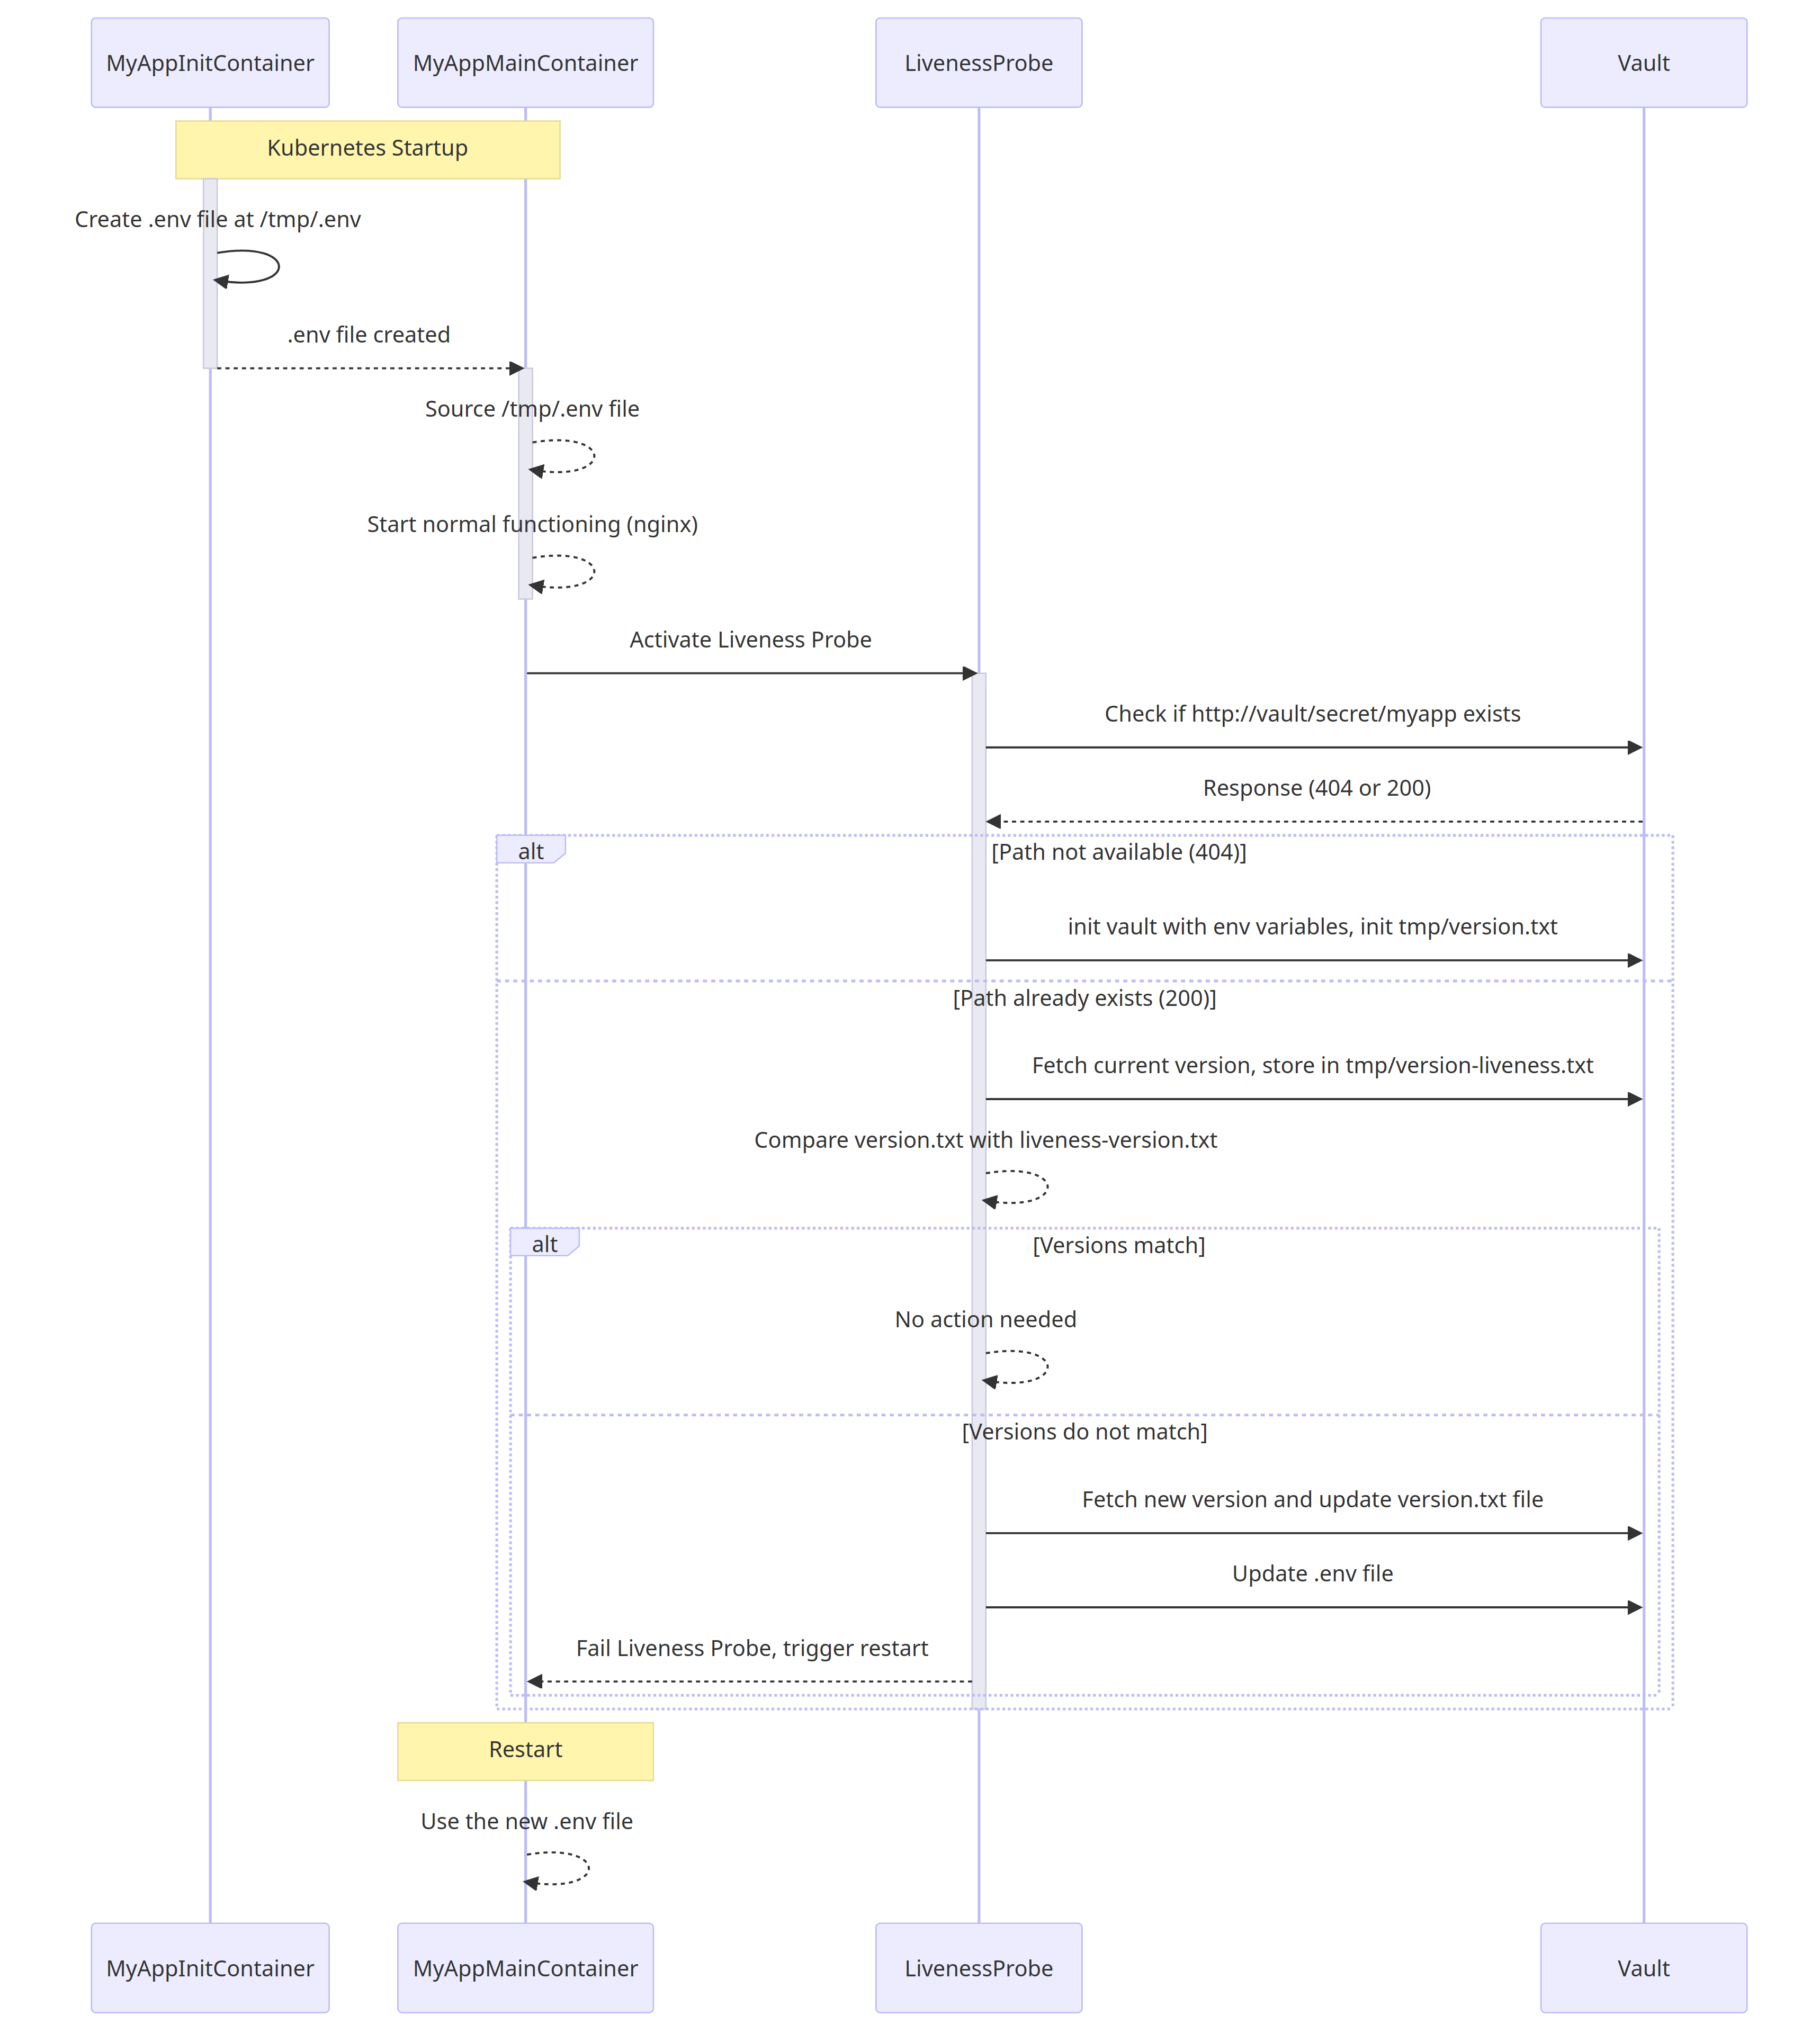
\includegraphics[width=0.8\linewidth]{figures/seq.png}
    \caption{implementation Sequence diagram}
    \label{fig:Sequence diagram}
\end{figure}

\subsection{Kubernetes and Vault Integration}

The script provided facilitates the integration between Kubernetes and HashiCorp Vault. It begins by checking if the \texttt{VAULT\_ENABLE} environment variable is set to "true". If enabled, it proceeds to fetch secrets from Vault using the specified token and address constructed based on environment variables (\texttt{VAULT\_SERVICE\_HOST} and \texttt{VAULT\_SERVICE\_PORT}). The script then handles various HTTP status codes returned by Vault API calls, such as 404 for a missing secret store or 403 for an incorrect token. Additionally, it supports initializing a new secret store if not found, exporting retrieved secrets as environment variables, and updating them as needed.

\subsection{Liveness Probe Implementation}

The liveness probe implementation leverages Kubernetes' built-in feature to ensure the health of containerized applications. Within the script, an HTTP request is made to the specified Vault address to check the availability of secrets. The response status code is evaluated, and actions are taken accordingly. If the secret store is missing (404), it initializes a new store. If the token is incorrect (403), it logs an error. Otherwise, it compares the version of the retrieved secrets with the locally stored version. If a mismatch is detected, it updates the environment variables and exports them for the application to use.

\subsection{Deployment Restart Mechanism}

The deployment restart mechanism is triggered conditionally based on the outcome of the liveness probe. If the script detects changes in the environment variables fetched from Vault, it exits with a non-zero status code (1), indicating that a restart is required. This triggers Kubernetes to restart the pod, ensuring that the application picks up the updated environment variables. Conversely, if no changes are detected, the script exits with a zero status code (0), indicating that the environment variables are up to date, and no restart is necessary. This mechanism ensures that the application remains resilient to configuration drifts and always uses the latest secrets from Vault.
